\documentclass{beamer}
\usepackage[utf8]{inputenc}
\usepackage{physics}
\usepackage[english,greek]{babel}
\usepackage{alphabeta}
\usepackage{amsmath, amssymb, amsfonts}
\usepackage{tikz, caption, subfig, comment, multicol, xcolor, tikz-feynman, tensor, graphics, graphicx, slashed, xfrac, biblatex, braket, siunitx, multirow, multicol, hyperref}

\usefonttheme[onlymath]{serif}
% \setsansfont{TeX Gyre Termes}

\addbibresource{references.bib}
\usetheme{Madrid}
\usecolortheme{default}


\title[\href{https://summerstudent.web.cern.ch/home}{CERN Summer Student Programme 2023}]
{     
      New kinematic weighting algorithm for CP asymmetries in charm decays
}
\setbeamerfont{footnote}{size=\tiny}
\setbeamerfont{caption}{size=\tiny}

\author[\href{https://github.com/GiorgosChr}{Georgios Christou}]
{Georgios Christou
\\
Supervisors: Dr.\@ Federico Betti and Prof.\@ Angelo Carbone}

\institute[\href{https://lhcb.web.cern.ch/}{LHCb}]
{
      LHCb Collaboration
}

\date{August 29, 2023}

% \logo{
\includegraphics[height=0.7cm]{../.images/Lhcb-logo-new.svg.png}}
\logo{\href{https://lhcb.web.cern.ch/}{
\includegraphics[height=0.7cm]{../.images/Lhcb-logo-new.svg.png}}}


\AtBeginSection[]{
  \begin{frame}
    \tableofcontents[currentsection]
  \end{frame}
}


\begin{document}
\selectlanguage{english}
\frame{\titlepage}
\begin{frame}
      \tableofcontents
\end{frame}

\section{Introduction}
\subsection{Asymmetries at the LHCb}

\begin{frame}
      \frametitle{\insertsubsectionhead}
      \rightarrow We study CP asymmetries in the following charm decays
      \begin{eqnarray*}
            &D^{\star+}\to D^0\pi^+ \text{ and } D^{\star-}\to \bar{D}^0\pi^-, \nonumber\\
            &D^0 \to K^-K^+ \text{ and } D^0 \to \pi^-\pi^+
    \end{eqnarray*}
      \textbf{At LHCb we observe:}
      \begin{itemize}
            \item CP asymmetry $A_{CP}$ \rightarrow Differences in matter and anti-matter decays
            \item Production asymmetry $A_{P}$ \rightarrow Differences in $D^{\star\pm}$ production
            \item Detection asymmetry $A_{D}$ \rightarrow Differences in $\pi_s^{\pm}$ detection
      \end{itemize}
      \bigbreak
      \rightarrow We mainly focus on CP and detection asymmetries throughout this project
\end{frame}

\begin{frame}
      \frametitle{\insertsubsectionhead}
      \rightarrow At an experiment our physical observable is the total asymmetry
      \begin{equation*}
            A_\text{total} = \frac{A_{CP} + A_{D}}{1 + A_{CP}A_D}\approx A_{CP} + A_{D} + \mathcal{O}(10^{-6})
      \end{equation*}
      where the asymmetries are $\mathcal{O}(10^{-3})$
      \begin{equation*}
            A_{D} = \frac{\int \dd \vec{p} N(\vec{p})A(\vec{p})}{\int \dd \vec{p} N(\vec{p})}\to \text{ Integrated detection asymmetry}
      \end{equation*}
      \begin{itemize}
            \item $N(\vec{p})$ \rightarrow Kinematic dependent distribution of $\pi_s$
            \item $A(\vec{p})$ \rightarrow Momentum dependent detection asymmetry
      \end{itemize}
      \rightarrow The total asymmetry is
      \begin{equation*}
            A_\text{total} = \frac{N_+ - N_-}{N_+ + N_-}
      \end{equation*}
\end{frame}

\begin{frame}
      \frametitle{\insertsubsectionhead}
      \rightarrow We define the total asymmetry difference
      \begin{equation*}
            \Delta A_\text{total} = A_\text{total}^{KK} - A_\text{total}^{\pi\pi} = \Delta A_{CP} + \Delta A_{D}
      \end{equation*}
      \rightarrow $\Delta A_D = 0$ if $N(\vec{p})$ is equal between the two decay modes

      \textbf{How can we obtain $\Delta A_{CP}$?}
      \begin{itemize}
            \item We need to equalize $D^0$ kinematic distributions for $D^0\to K^-K^+$ and $D^0\to \pi^-\pi^+$ decay modes
            \item The following weighting function allows us to do that
      \end{itemize}
      \begin{equation*}
            Q(\vec{p}_{D^\star}, \vec{p}_{\pi_s}) \simeq \frac{\Gamma_{D^0}^{\pi\pi}(\vec{p}_{D^\star} - \vec{p}_{\pi_s}) + \Gamma_{\bar{D}^0}^{\pi\pi}(\vec{p}_{D^\star} - \vec{p}_{\pi_s})}{\Gamma_{D^0}^{KK}(\vec{p}_{D^\star} - \vec{p}_{\pi_s}) + \Gamma_{\bar{D}^0}^{KK}(\vec{p}_{D^\star} - \vec{p}_{\pi_s})}\text{, Ref: [\href{https://indico.cern.ch/event/780618/\#-update-of-delta-a_cp-to-the}{1}, \href{https://groups.cern.ch/group/lhcb-phys-charm/Lists/Archive/Flat.aspx?RootFolder=/group/lhcb-phys-charm/Lists/Archive/Some\%20thoughts\%20on\%20DeltaACP&FolderCTID=0x012002009FBA6738F0FB684B8D8EB7AE0A048769}{2}]}
      \end{equation*}
      

      \bigbreak
      \to This weighting function works if $A_D(\vec{p}) < 0.2$, thus we apply fiducial cuts to remove regions associated with larger detection asymmetries ($\sim 30\%$ of data sample) for analysis performed on real data
\end{frame}

\begin{frame}
      \frametitle{\insertsubsectionhead}
      \begin{figure}
            \centering
            \subfloat{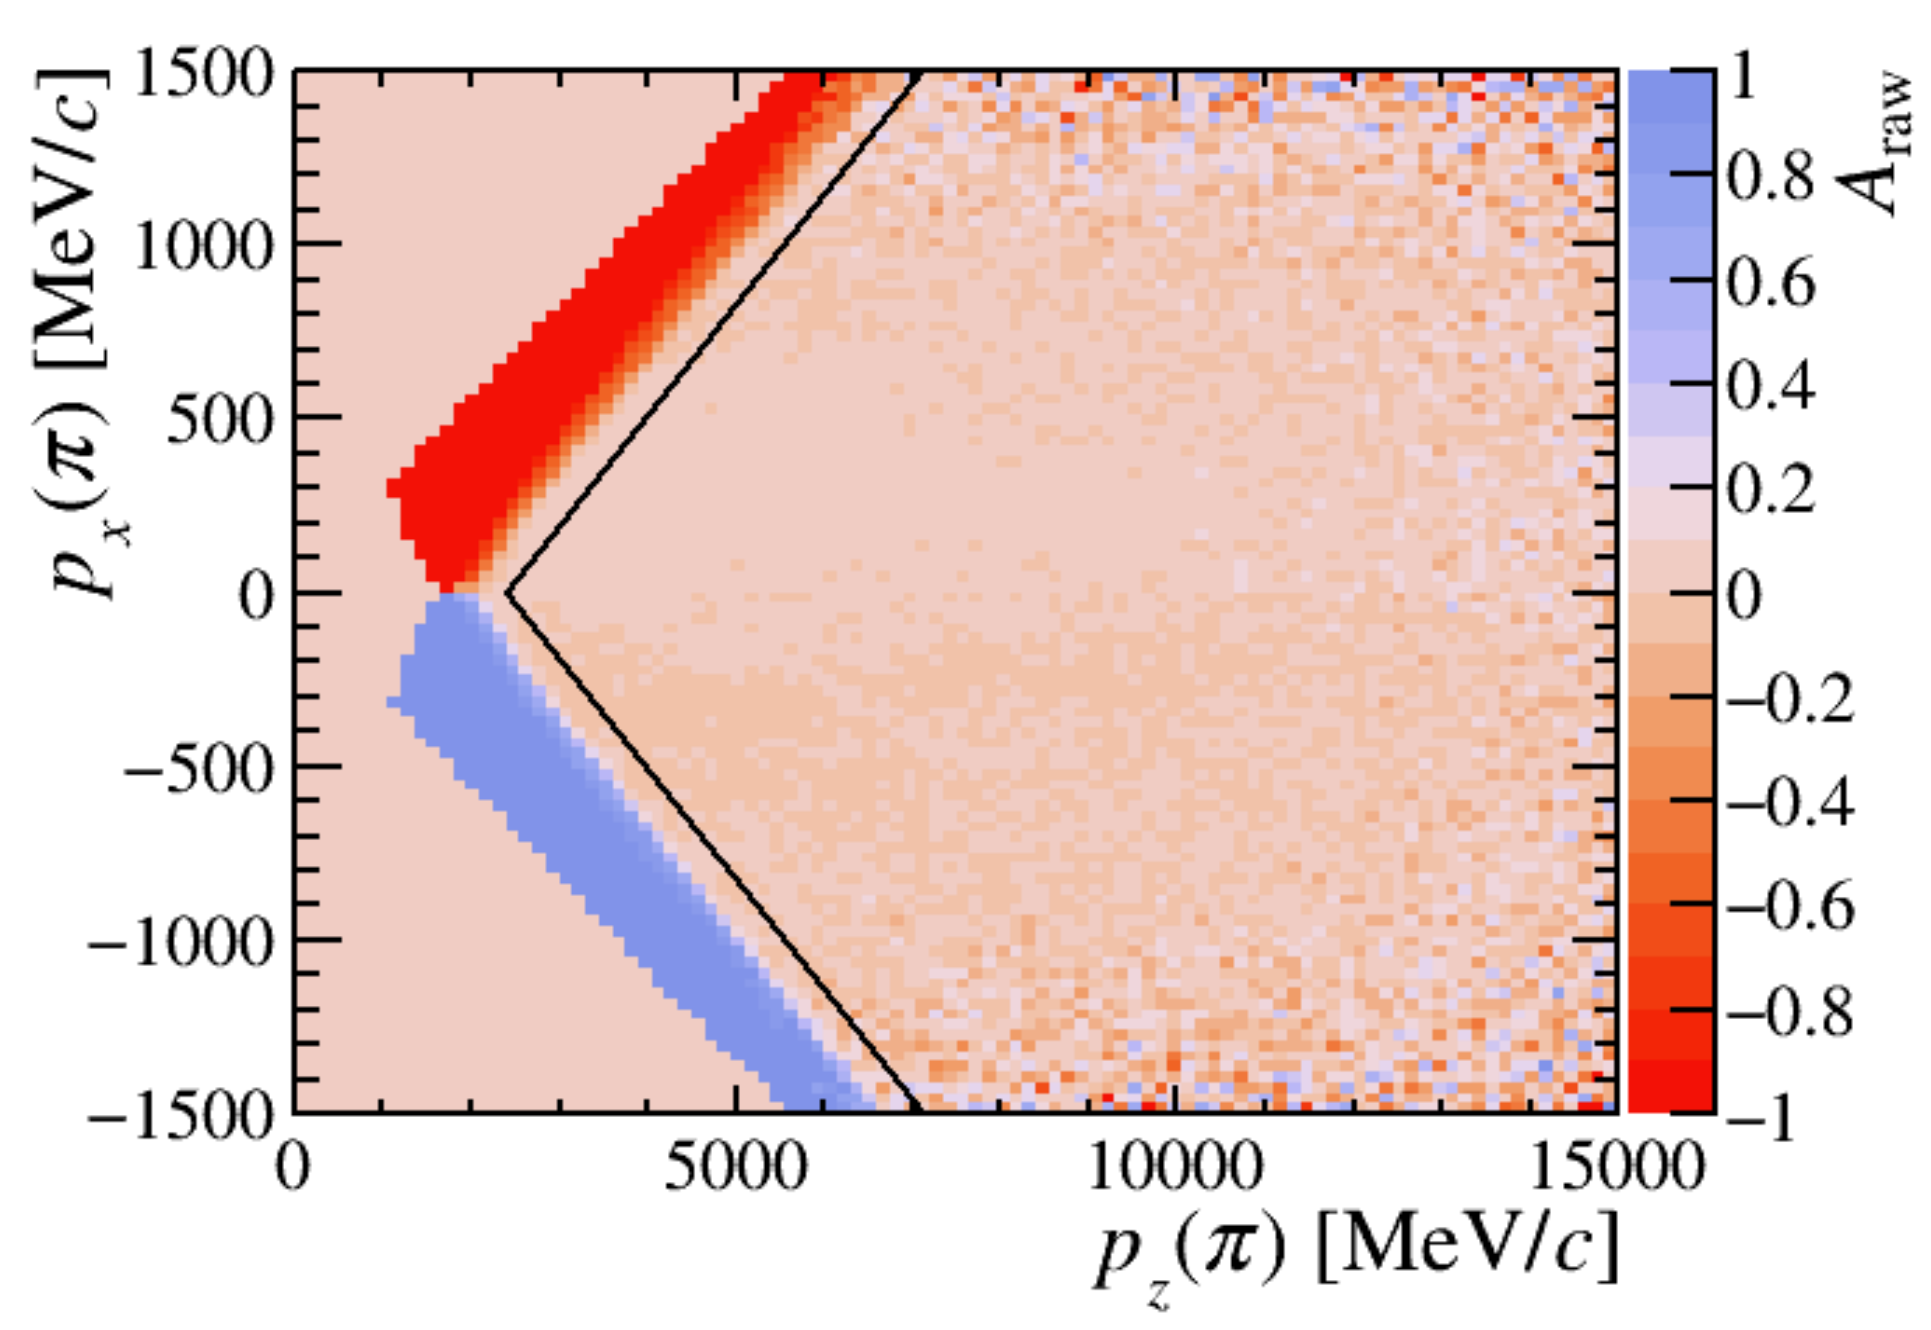
\includegraphics[width = 0.5\textwidth]{Figures/Screenshot from 2023-08-30 18-36-02.png}}
            \subfloat{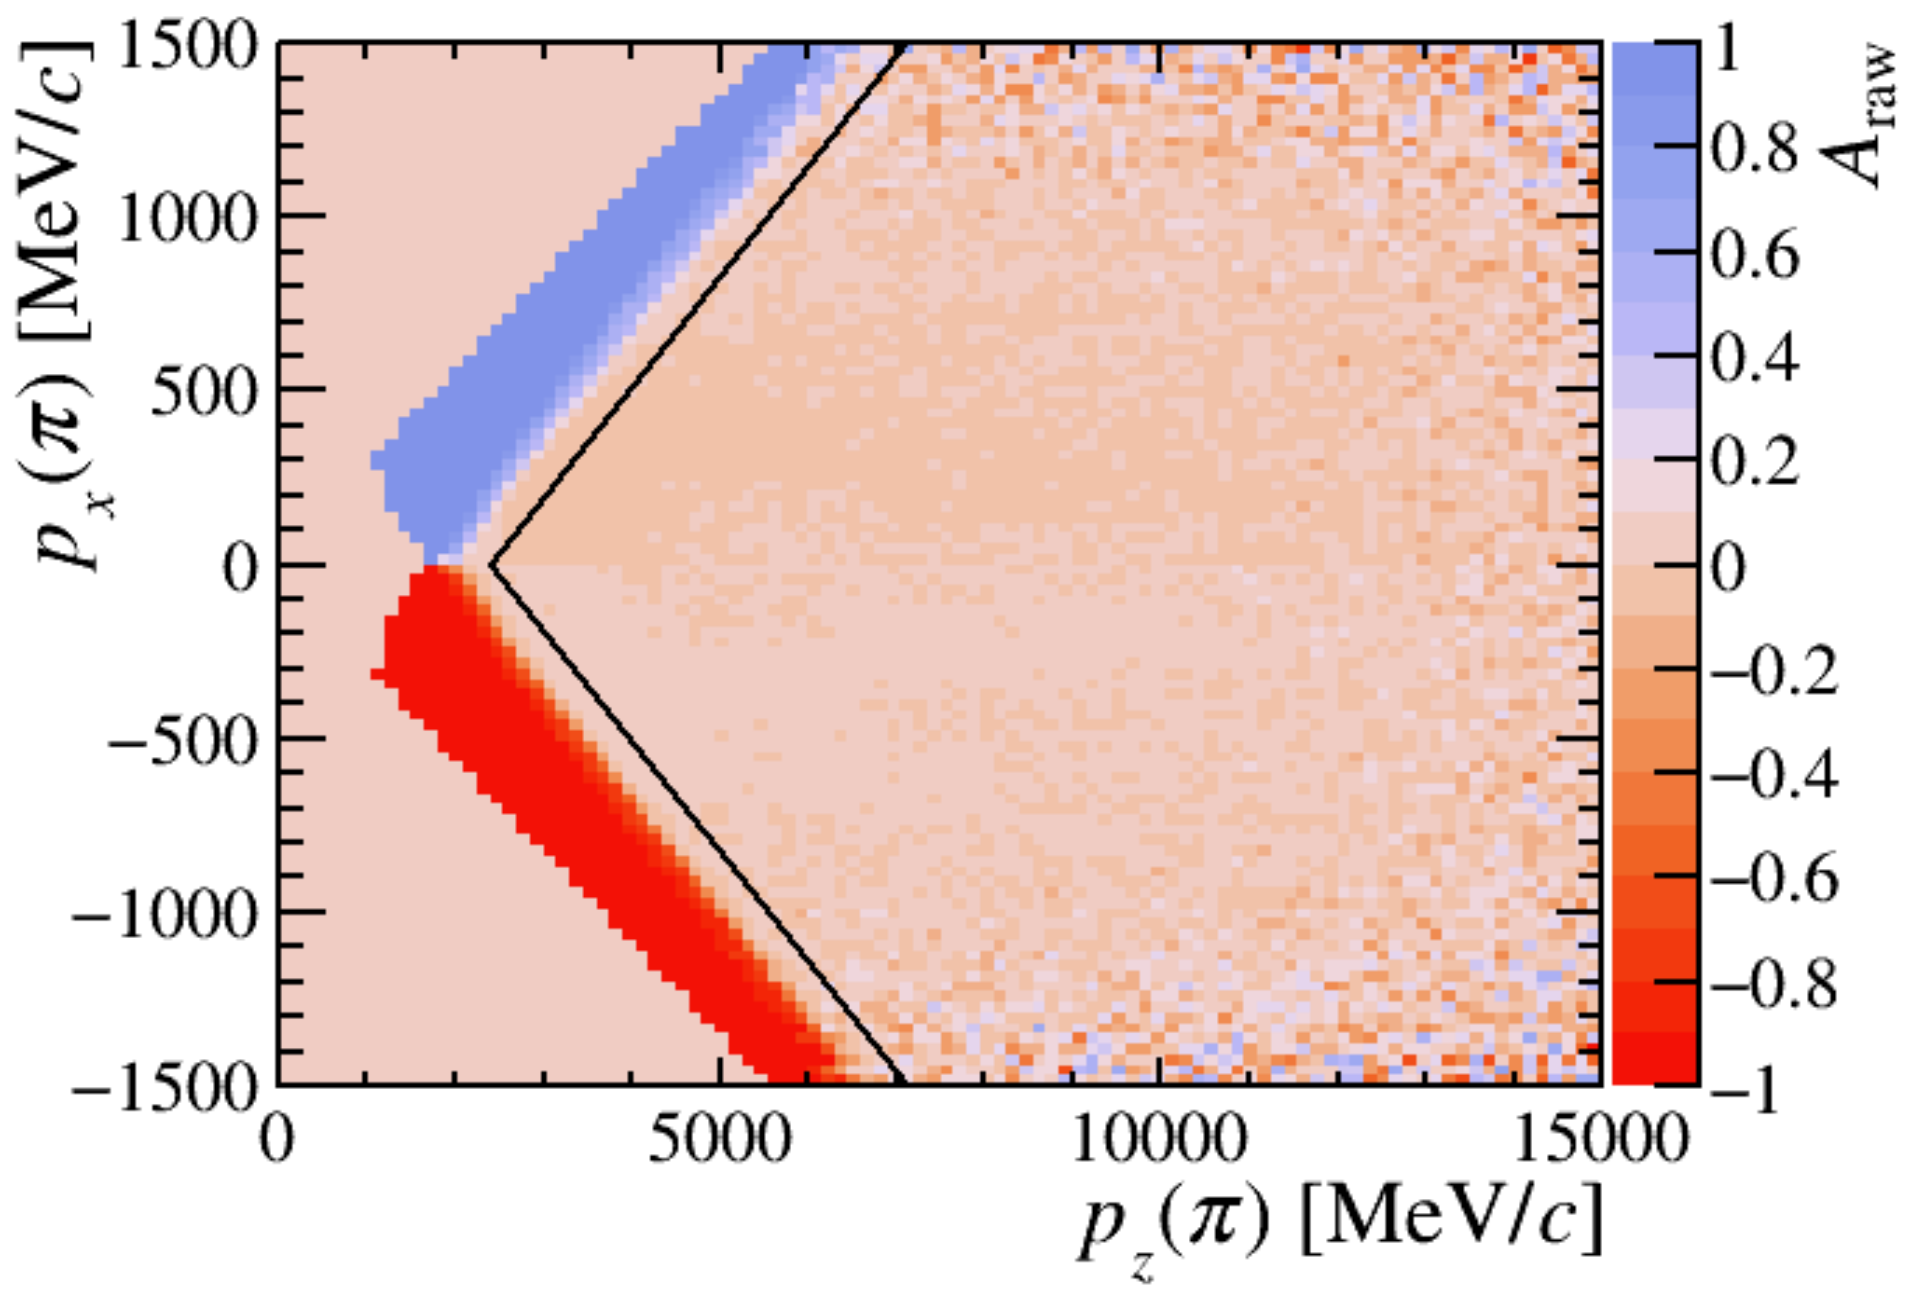
\includegraphics[width = 0.5\textwidth]{Figures/Screenshot from 2023-08-30 18-36-17.png}}
      \end{figure}
\end{frame}

\begin{frame}
      \frametitle{\insertsubsectionhead}
      \rightarrow We introduce a new weighting technique Ref: [\href{https://indico.cern.ch/event/780618/\#-update-of-delta-a_cp-to-the}{1}, \href{https://groups.cern.ch/group/lhcb-phys-charm/Lists/Archive/Flat.aspx?RootFolder=/group/lhcb-phys-charm/Lists/Archive/Some\%20thoughts\%20on\%20DeltaACP&FolderCTID=0x012002009FBA6738F0FB684B8D8EB7AE0A048769}{2}]
      \begin{equation*}
            Q(\vec{p}_{D^0}) \simeq \frac{\Gamma_{D^0}^{\pi\pi}(\vec{p}_{D^0}) + \Gamma_{\bar{D}^0}^{\pi\pi}(\vec{p}_{D^0})}{\Gamma_{D^0}^{KK}(\vec{p}_{D^0}) + \Gamma_{\bar{D}^0}^{KK}(\vec{p}_{D^0})}\to \text{Not affected by }A_D
      \end{equation*}
      \rightarrow $\Gamma_{D^0/\bar{D}^0}^{\pi\pi/ KK}(\vec{p}_{D^0/\bar{D}^0})$ for untagged $D^0$ candidates

      \rightarrow Even if high $A_D(\vec{p})$ regions are present $\Delta A_D = 0$
      \bigbreak
      \rightarrow Now we can use the sample that was previously removed by fiducial cuts\Rightarrow \textbf{More statistics!}
      \begin{equation*}
            \boxed{\Delta A_\text{total} = \Delta A_{CP}}
      \end{equation*}
      % \bigbreak 
      {\bf However:}
      \begin{itemize}
            \item The untagged $D^0$ candidates were not kept in Run-2
            \item The untagged $D^0$ candidates are kept in Run-3, but we do not have enough statistics
      \end{itemize}
      \rightarrow We use MC samples to test the new weighting technique
\end{frame}

\section{Analysis}
\subsection{RapidSim}

\begin{frame}
      \frametitle{\insertsubsectionhead}
      \rightarrow We generate data using RapidSim and introduce:
      \begin{itemize}
            \item Different CP asymmetries for $D^0\to K^-K^+$ and $D^0\to\pi^-\pi^+$ decay modes $\left(A_{CP}^{KK} = 0.1,\; A_{CP}^{\pi\pi} = 0.2,\; \rightarrow \Delta A_\text{total} = -0.1\right)$
            \item The same $A_D(\vec{p}) = 100\%$ in specific regions$^*$ \\ \rightarrow The integrated detection asymmetries are different for the two samples because the kinematic distributions differ
      \end{itemize}
      % \rightarrow We exclude negative $\pi_s$ \Rightarrow Large detection asymmetry
      \rightarrow We have around 4.8 ($K^-K^+$ mode) and 4.2 ($\pi^-\pi^+$ mode) million events
      \begin{figure}
            \centering
            \subfloat{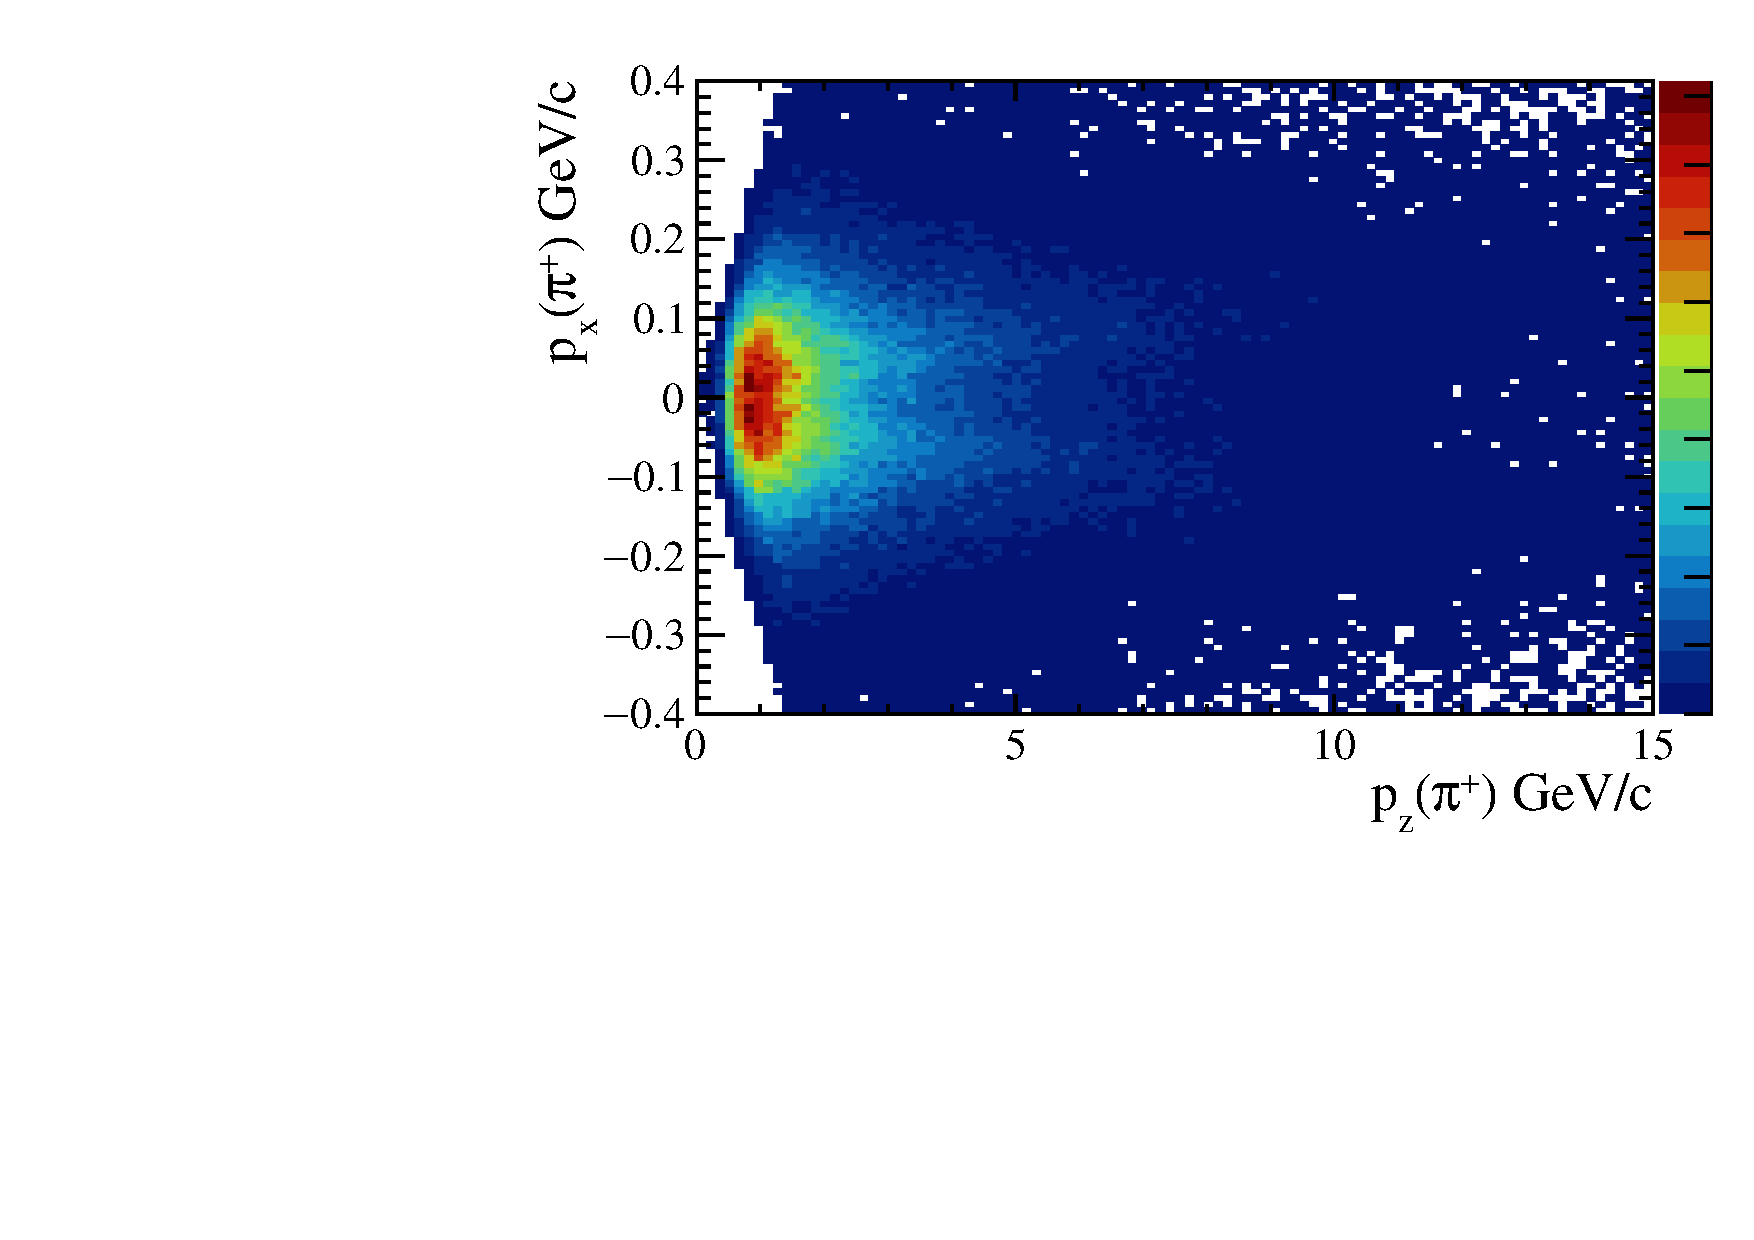
\includegraphics[width = 0.4\textwidth]{../work/RapidSimAnalysis/MomentumDependence/Plots/KK_Dst_PXPZ_Positive.pdf}}
            \subfloat{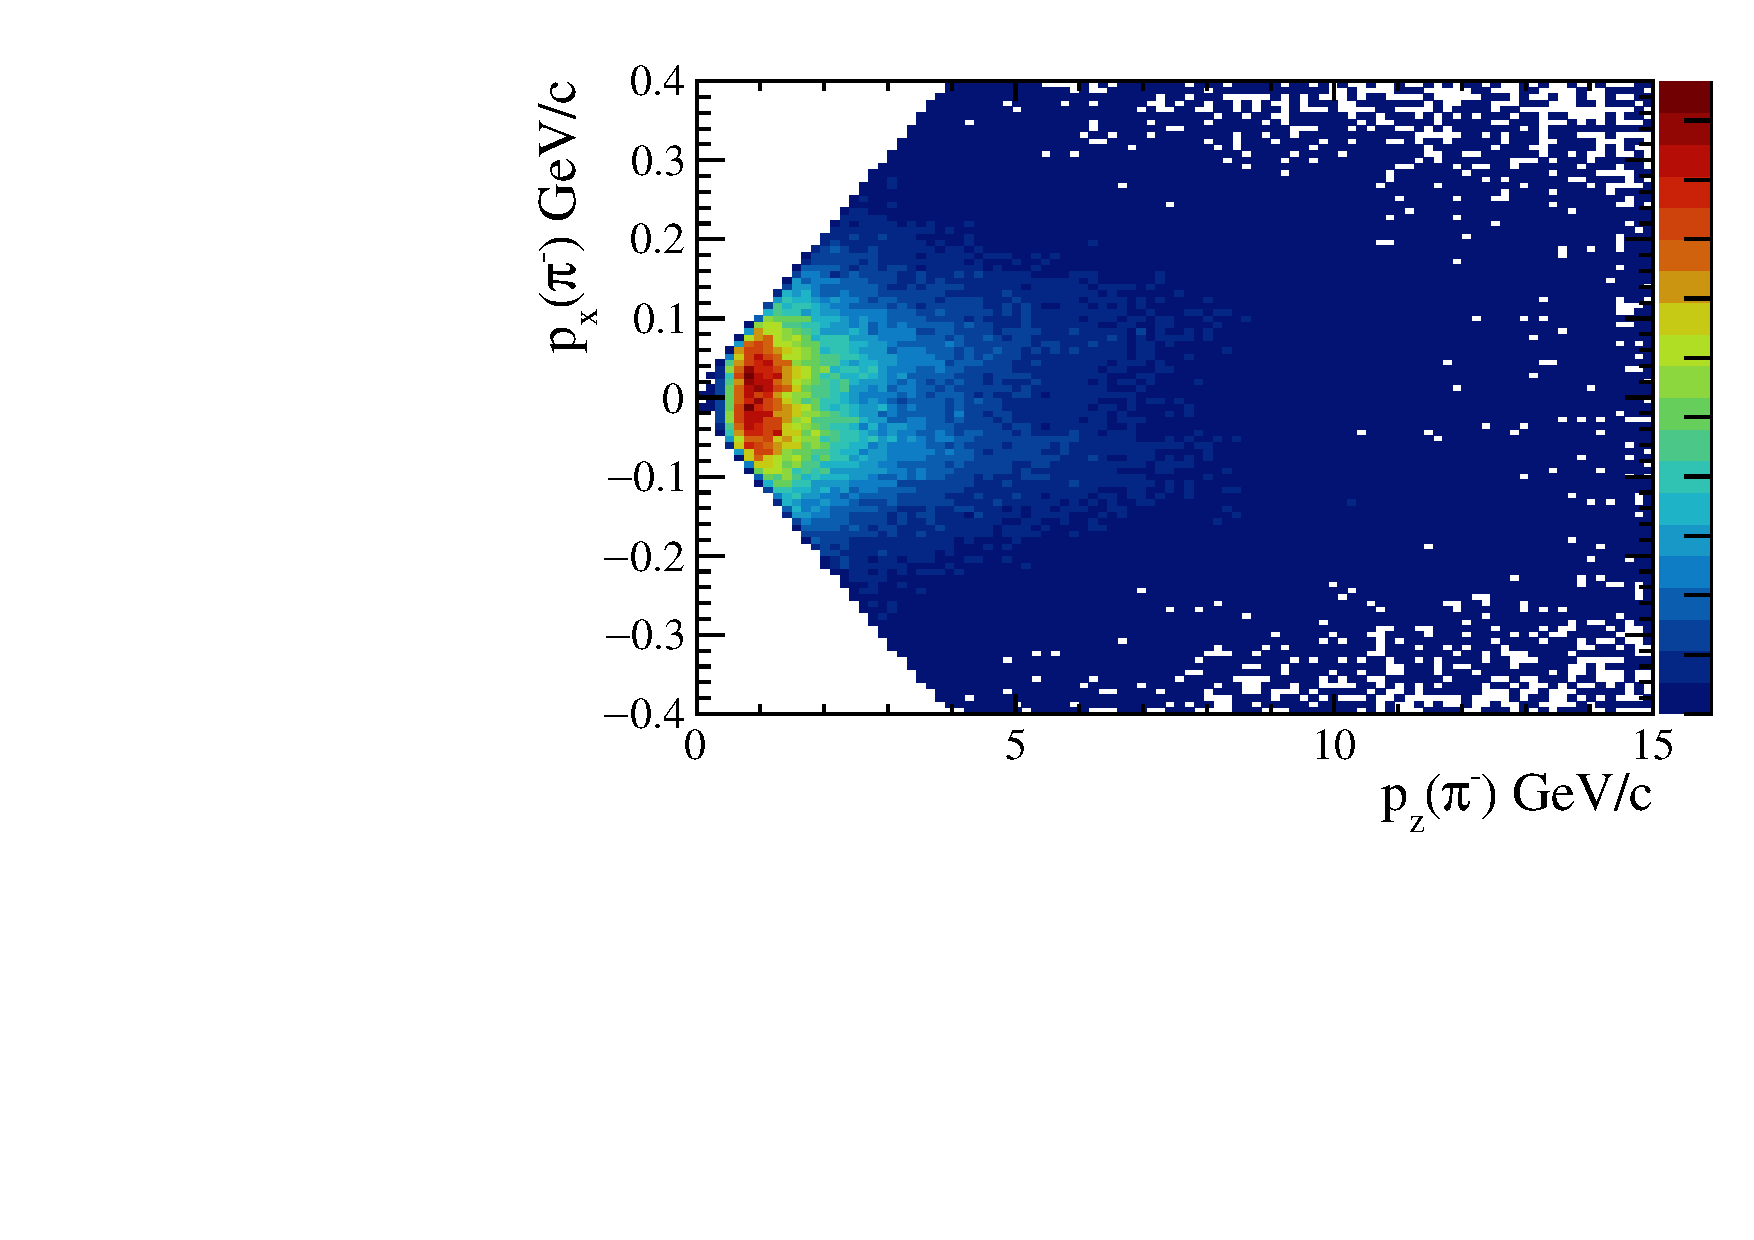
\includegraphics[width = 0.4\textwidth]{../work/RapidSimAnalysis/MomentumDependence/Plots/KK_Dst_PXPZ_Negative.pdf}}
      \end{figure}
      \scriptsize
      $^*$ This is an extreme case which is different from what we observe with real data
\end{frame}

\begin{frame}
      \frametitle{\insertsubsectionhead}
      \rightarrow We calculate the weighting function before and after the introduction of the detection asymmetry
      \begin{itemize}
            \item Before: Emulates $D^0$ not associated with $\pi_s$ \Rightarrow New weighting technique
            \item After: Emulates $D^0$ associated with $\pi_s$ \Rightarrow Standard technique
      \end{itemize}
      \begin{center}
            \scriptsize
            \begin{tabular}{c|c|c|c}
                  Technique& & Weighted & Unweighted\\
                  \hline\hline
                  \multirow{2}{*}{Not associated} & $\Delta A_\text{total}$ & $-0.09845 \pm 0.00073$ & \\
                  & Deviation $(\sigma)$ & $2.12$ & $-0.08303 \pm 0.00072$\\
                  \cline{1-3}
                  \multirow{2}{*}{Associated with $\pi_s$} & $\Delta A_\text{total}$ & $-0.09578 \pm 0.00073$ & $23.6$\\
                  & Deviation $(\sigma)$ & $5.78$ & \\
          \end{tabular}
    \end{center}
    \normalsize
    \begin{itemize}
      \item The unweighted calculation is biased as expected \rightarrow $\Delta A_D \neq 0$
      \item The weighting function with $\pi_s$ association yields a biased result
      \item The new weighting technique (not affected by large $A_D(\vec{p})$) allows us to keep events associated with large $A_D(\vec{p})$ \Rightarrow {\bf More statistics!}
    \end{itemize}
\end{frame}

\subsection{Particle Gun}

\begin{frame}
      \frametitle{\insertsubsectionhead}
      \rightarrow We use Particle Gun data for a more realistic scenario.
      \begin{itemize}
            \item We do not introduce CP asymmetry $\Delta A_{CP} = 0$
            \item The detection asymmetry is the one expected in data
      \end{itemize}
      \begin{figure}
            \centering
            \subfloat{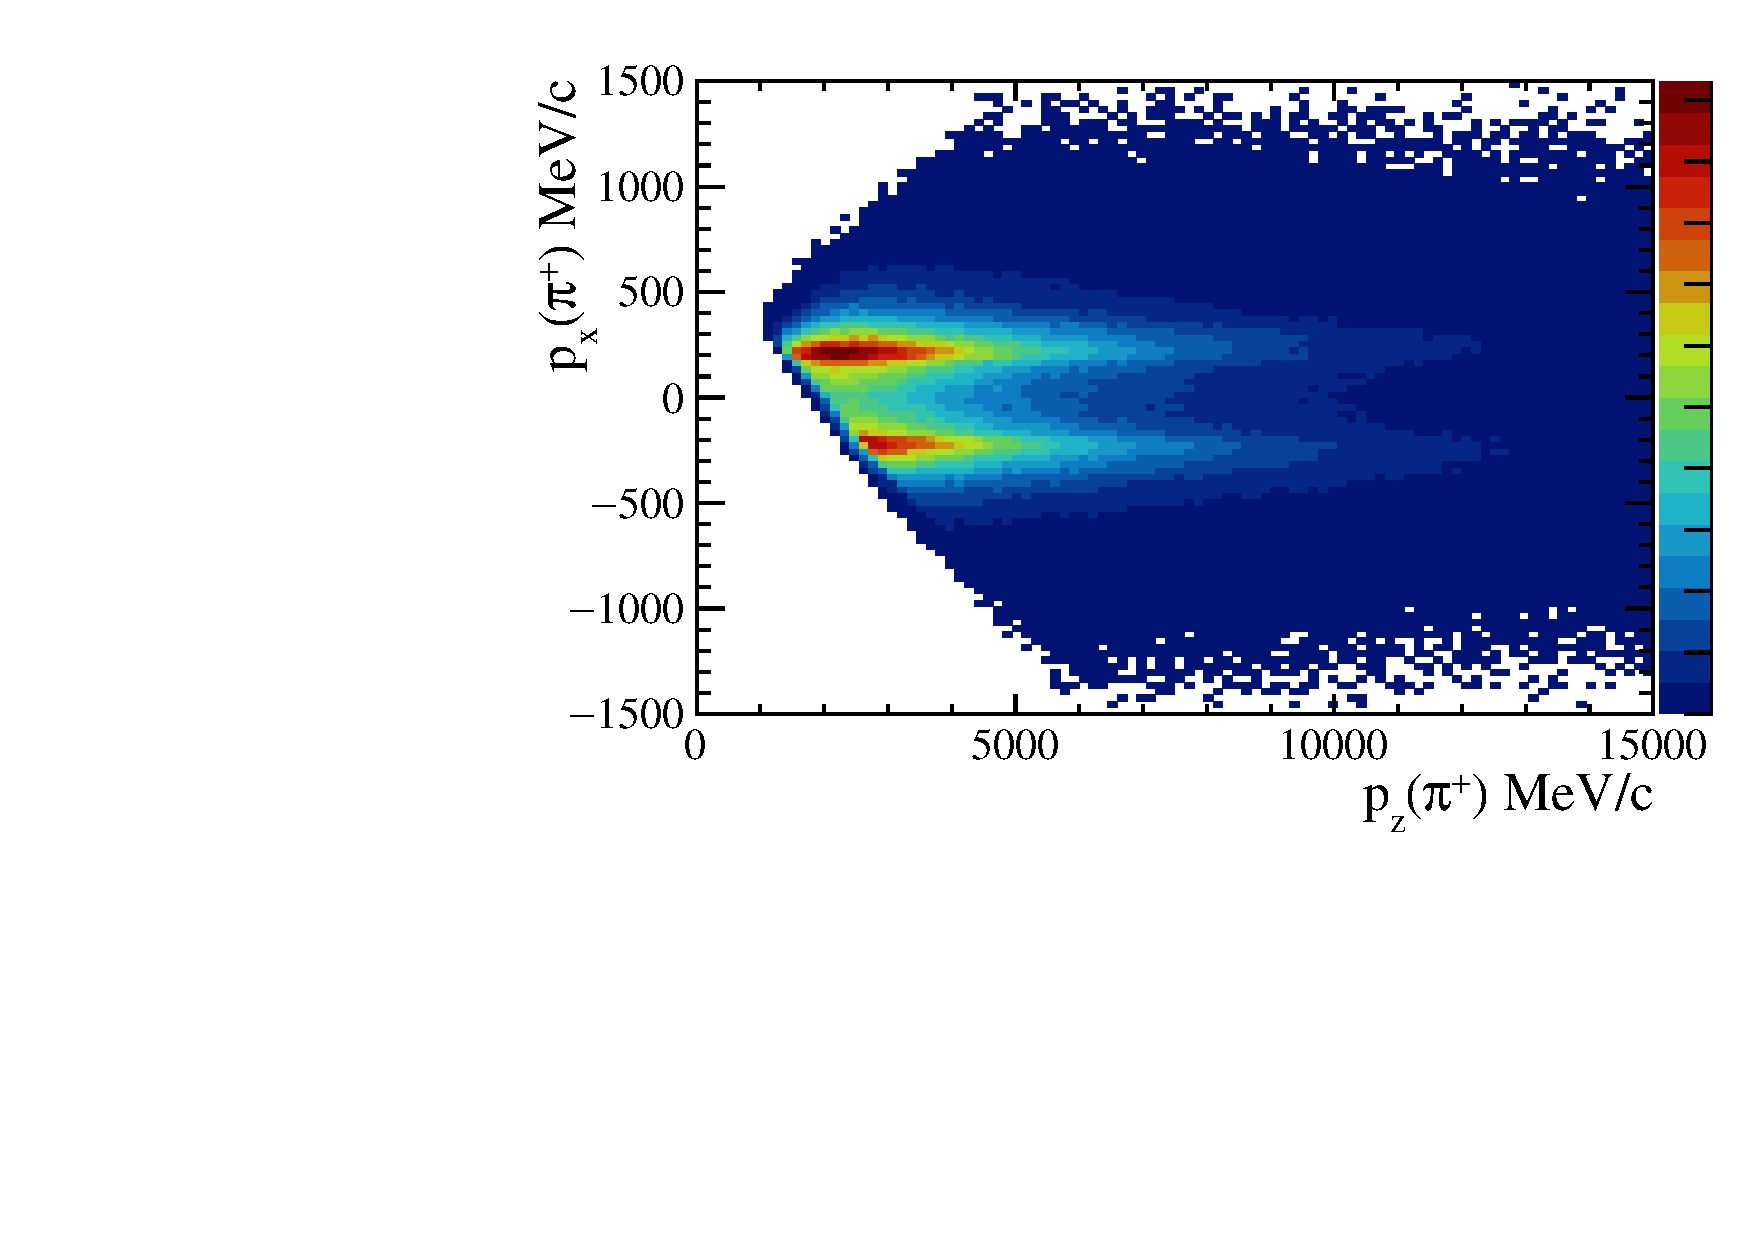
\includegraphics[width = 0.42\textwidth]{../work/RapidSimAnalysis/PGunAnalysis/Plots/KK_Dst_PXPZ_Positive.pdf}}
            \subfloat{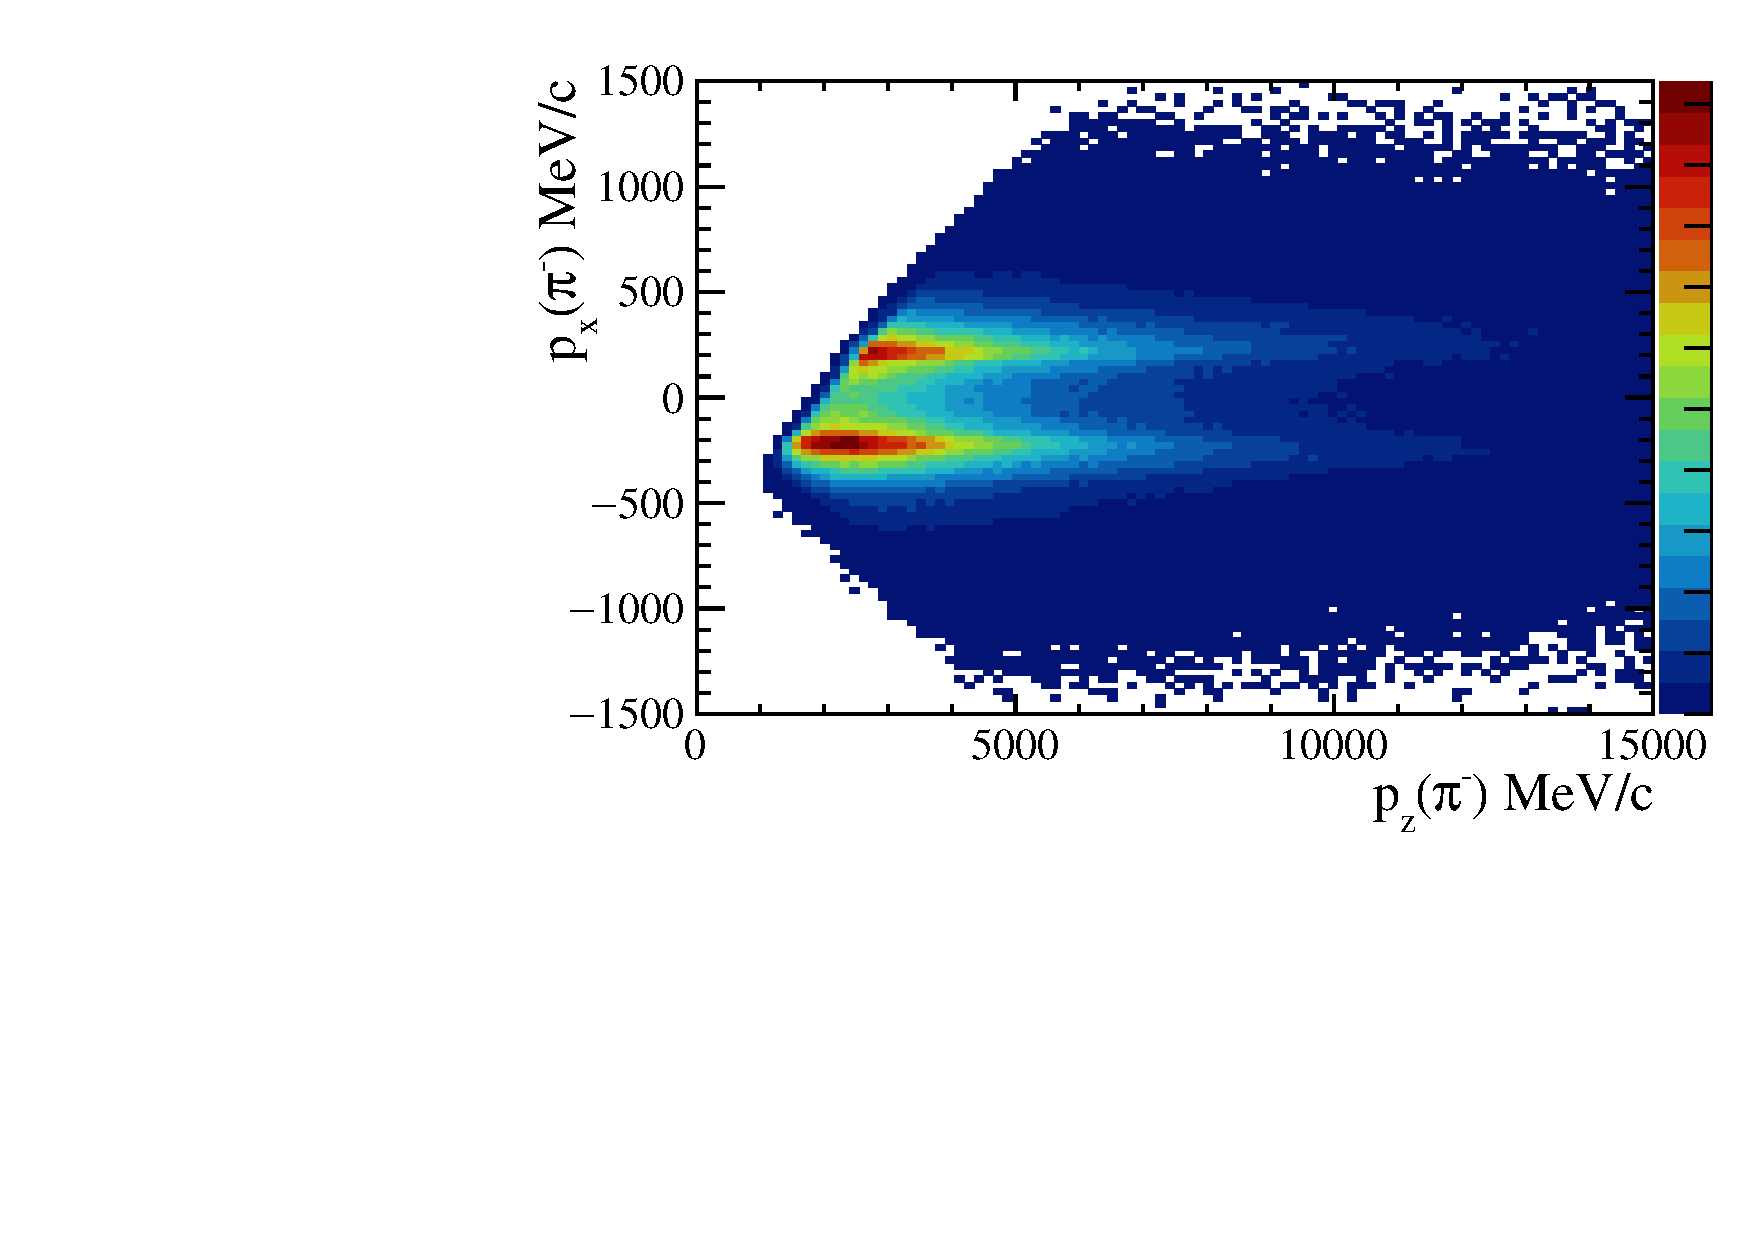
\includegraphics[width = 0.42\textwidth]{../work/RapidSimAnalysis/PGunAnalysis/Plots/KK_Dst_PXPZ_Negative.pdf}}
      \end{figure}
      \rightarrow The new weighting technique should yield $\Delta A_\text{total} = 0$
\end{frame}

\begin{frame}
      \frametitle{\insertsubsectionhead}
      \begin{center}
            \scriptsize
            \begin{tabular}{c|c|c|c}
                  Technique & & Weighted & Unweighted\\
                  \hline\hline
                  \multirow{2}{*}{Not associated} & $\Delta A_\text{total}$ & $-0.000084\pm 0.000262$& \\
                  & Deviation $(\sigma)$ & $0.32$& $-0.000015\pm 0.000262$\\
                  \cline{1-3}
                  \multirow{2}{*}{Associated with $\pi_s$} & $\Delta A_\text{total}$ & $-0.000036\pm 0.000262$& $0.057$\\
                  & Deviation $(\sigma)$ & $0.14$& \\
            \end{tabular}
      \end{center}
      \normalsize
      \begin{itemize}
            \item The effect of $A_D$ is small
            % \item The asymmetries cancel out after averaging both magnet polarities
            \item With these statistics we do not see any improvement
            \item The measurements seems unbiased even without any weighting applied
      \end{itemize}
\end{frame}

\section{Conclusions}
\begin{frame}
      \frametitle{\insertsectionhead}
      \textbf{RapidSim:}
      \begin{itemize}
            \item The old weighting function reduces the deviation of $\Delta A_\text{total}$, however it still introduces bias to our results
            \item The new weighting technique reduces the deviation of $\Delta A_\text{total}$ and allows us to keep all events, thus using higher statistics\Rightarrow \textbf{More effective}
      \end{itemize}
      \bigbreak
      \textbf{Particle Gun:}
      \begin{itemize}
            \item The effect of $\Delta A_D$ is small
            % \item The averaging of both magnet polarities removes the effect
            \item With this statistics, we do not see any significant improvement
      \end{itemize}
      \bigbreak
      \textbf{Next steps:}
      \begin{itemize}
            \item Look at Run-3 data
      \end{itemize}
\end{frame}


\begin{frame}
      \LARGE
      \centering
      Thank you for your attention!

      Questions?
\end{frame}
\end{document}